
\section*{SiPMWheel: a large-area, position-sensitive, energy-resolving light collector (Asaadi, Jones and Nygren.)}

\section{Introduction}

The designs of scintillation light collection systems for noble element time projection chambers (TPCs) are driven by two main requirements:

\begin{itemize}
\item Photons with very short wavelengths (128 nm in Ar, 175 nm in Xe) must be collected.
\item Large surface areas must be instrumented to collect as much light as possible, with a channel count kept low in order not to drive up the system cost.
\end{itemize}

Although some VUV-sensitive light detectors are available \cite{Zabrodskii2015348,DeepUV}, their quantum efficiency at these wavelengths is typically not high, and their surface area per channel is not large.  To sensitize visible light detectors to VUV photons a wavelength shifter is often employed, absorbing in the UV and emitting in the visible.  A common choice is tetra-phenyl butadiene (TPB) \cite{Baptista:2013gna,Hanagodimath2008,Gehman:2013lsx,Gehman:2011xm,Burton1973,Jones:2012hm,Francini:2013Jinst}.  A fraction of the visible light thus emitted can then be detected by a standard photon detector like a silicon photomultiplier (SiPM) or a photomultiplier tube (PMT).  Several geometries have been considered, including through-plate systems \cite{Briese:2013wua,PostdocRevisited}, high-reflectivity foils \cite{Szelc:2013ooa,Kryczynski:2015pmj}, and light-guides \cite{Baptista:2012bf,Moss:2014ota,Mufson:2013zba}.  Light guide systems, have the advantage that large areas can be sensitized with only a moderate channel count.  However, it has the disadvantage that light losses through non totally-internally-reflected rays, and surface scattering and re-absorption effects \cite{Jones:2013sfa} are significant, and that the collection efficiency depends on the geometrical position of light arrival, making calorimetric reconstruction of localized events difficult.

We propose to develop a new large-area wavelength-shifting detector based on the light-guiding concept, with significantly improved collection efficiency and calorimetric performance.  This concept is motivated by the needs of the NEXT neutrinoless double beta decay experiment \cite{Mart} and by low energy physics analyses such as those of supernova neutrinos, proton decay and solar neutrinos in large liquid argon TPC detectors like DUNE \cite{Ankowski:2016lab,Kudryavtsev:2016ybl}. The pervasiveness of noble-element TPCs in particle physics is so widespread that light collection solutions with strong position and / or strong calorimetric resolution potential are likely to be widely applicable.  Use cases as a primary scintillation detector may include noble element dark matter searches and other surface and underground liquid argon TPC detectors, and as an electroluminescent energy plane may include the DUNE two-phase far detector and possible argon gas near detector.

\section{Research team, existing facilities, and details of request}

This project will be led by Profs. Jonathan Asaadi, Ben Jones, and David Nygren at UTA.  It will make use of existing liquid argon and high pressure xenon gas purification systems which are already operational at UTA and shown in Figure~\ref{fig:ExistingGasSystems}.  


\begin{figure}[t]
\begin{centering}
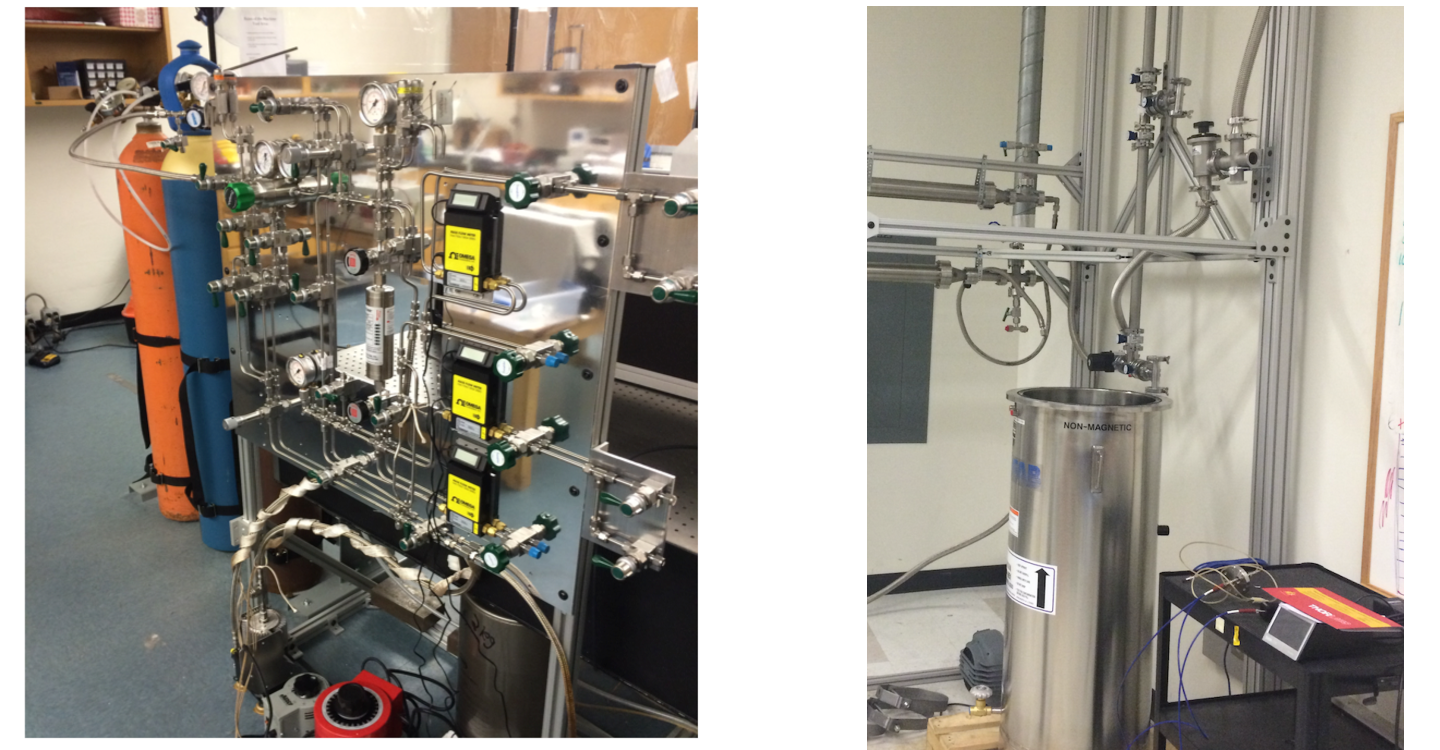
\includegraphics[width=0.90\columnwidth]{./images/PhotosOfLabs.pdf}
\par\end{centering}

\caption{Left: Existing high pressure xenon gas purification and recirculation system in the lab of Nygren and Jones.  Right: Existing liquid argon purification system in lab of Asaadi. \label{fig:ExistingGasSystems}}
\end{figure}

This project also leverages the experience of these researchers.  Nygren is the inventor of the time projection chamber \cite{Nygren:1976fe} and a pioneer of electroluminescent xenon detectors for neutrinoless double beta decay \cite{Gonzalez-Diaz:2015oba,Mart,Nygren:2009zz,Goldschmidt:2011ria,Nygren:2007zzc,Sinclair:2011zz}.  He is spokesperson of the NEXT collaboration and developed a test stand that demonstrated energy resolution near the intrinsic limit of xenon gas \cite{Alvarez:2012yxw} (1\% FWHM at 662 keV), the worlds most precise energy resolution from a xenon detector. Asaadi is a prominent member of the MicroBooNE \cite{Chen:2007ae}, SBND \cite{Antonello:2015lea}, DUNE \cite{Acciarri:2015uup} and LArIAT \cite{Cavanna:2014iqa} collaborations, with expertise in liquid argon TPC detector design, development and construction \cite{Asaadi:2014iva}.  Jones has extensive experience in noble element light collection,  including the developing ``Wunderbar'' light-guide detectors for large LArTPCs \cite{Jones:2013sfa,Baptista:2012bf,Moss:2014ota}; assembling and operating the Bo liquid argon optical test stand at Fermilab \cite{Jones:2013bca,Jones:2013mfa,Jones:2013nea}; exploring wavelength shifter properties and photochemistry \cite{Jones:2012hm}; and simulating light in liquid argon \cite{uBOpticalSim,Jones:2013sfa}.

Most supporting equipment for this project is already available or will be purchased from University funds, including the test stands, data acquisition systems and SiPMs, all of which were already acquired for other projects.  To pursue this research we request support for: 

\begin{enumerate}
\item  Personnel: one FTE graduate student (in the form of two students at 50\% effort level each), and one undergraduate.
\item  M\&S costs: to include argon and xenon supply, as well as fluors and plate materials.
\end{enumerate}



\section{Detection concept and comparison to existing devices \label{sec:concept}}

The detector we plan to develop will use an array of silicon photomultipliers (SiPMs) coupled around the perimeter of a TPB coated plate.  As with bar-type light-guide detectors (hereafter referred to as ``bars''), shown in Figure~\ref{fig:DetectorSketch}, top, VUV photons absorbed at the coating surface are re-emitted in the blue, some of them into the totally internally reflected modes of the polymer plate.  In contrast to bar detectors, the SiPMWheel is instrumented at many points around the perimeter.  This provides significant advantages which we hope to demonstrate: 1) the sensitive surface area is maximized relative to the allowed path-length between emission and detection, which optimizes light collection efficiency against losses during propagation; 2) the fraction of solid angle outside the totally internally reflected range is much reduced, leading to a higher trapped light yield  3) by reading out all SiPMs, geometrical information about the  event can be extracted - as well as being intrinsically useful, this position information allows for a correction to be applied to improve calorimetric response.




\begin{figure}[t]
\begin{centering}
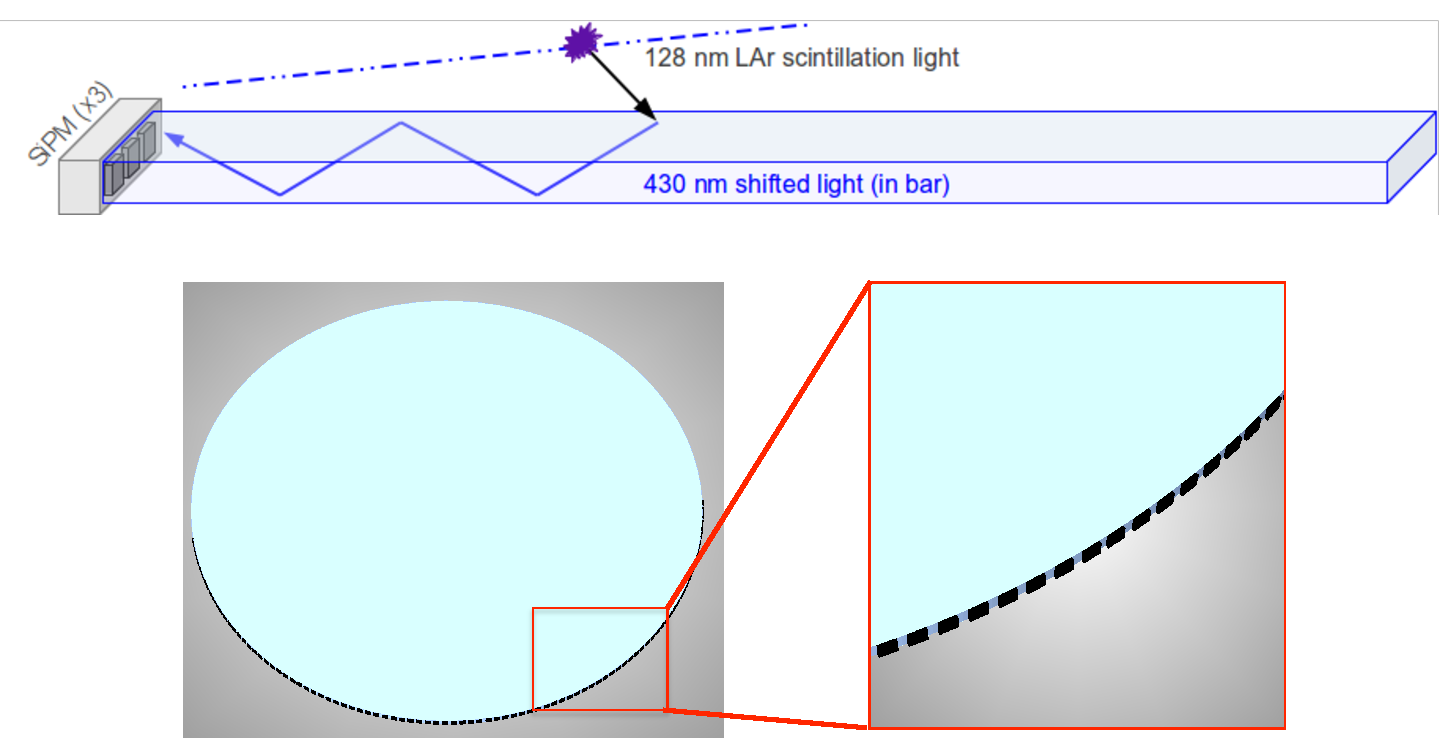
\includegraphics[width=0.95\columnwidth]{./images/SketchOfDetector.pdf}
\par\end{centering}

\caption{Top: Example of operation of bar detectors, like the ``Wunderbar'' - image from \cite{Whittington:2014aha}.  Bottom: Drawing of plate detector we propose to develop. \label{fig:DetectorSketch}}
\end{figure}

In this section we derive some quantitative comparisons between our proposed SiPMWheel detector and the more typical bar-type geometry.  We assume the same coating properties can be achieved over a 2D surface for both plates and bars (fabrication of the ``Wunderbar'' is easily generalizable \cite{Moss:2014ota}) and that the bar length / plate radius are free parameters to be optimized for each device. 

When comparing different light collection technologies it is important to define a useful Figure~of merit (FOM).  The following FOMs, though by no means exclusive, appear to represent reasonable ways to assess the light collector performances for our intended use cases:



\begin{figure}[t!]
\begin{centering}

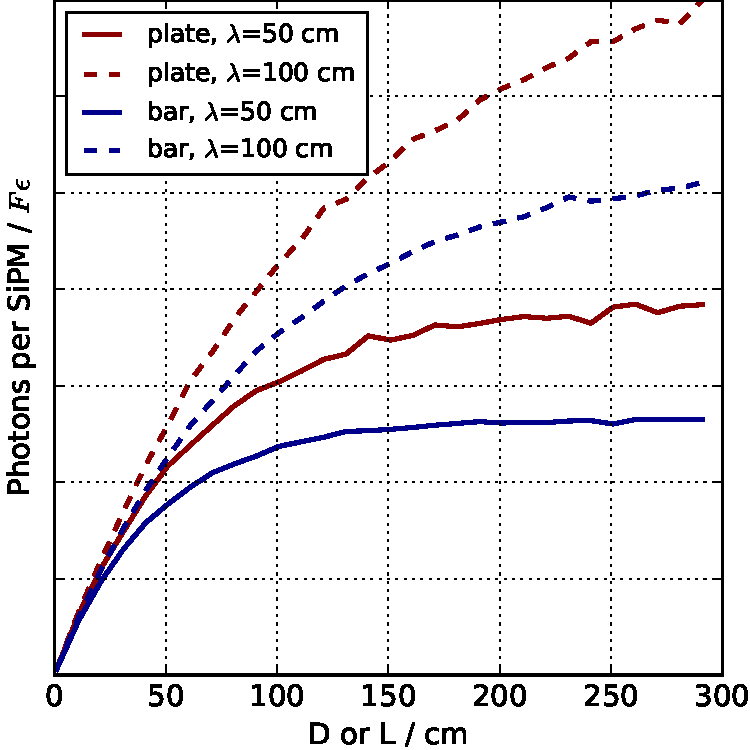
\includegraphics[width=0.48\columnwidth]{./images/FOM1.pdf}
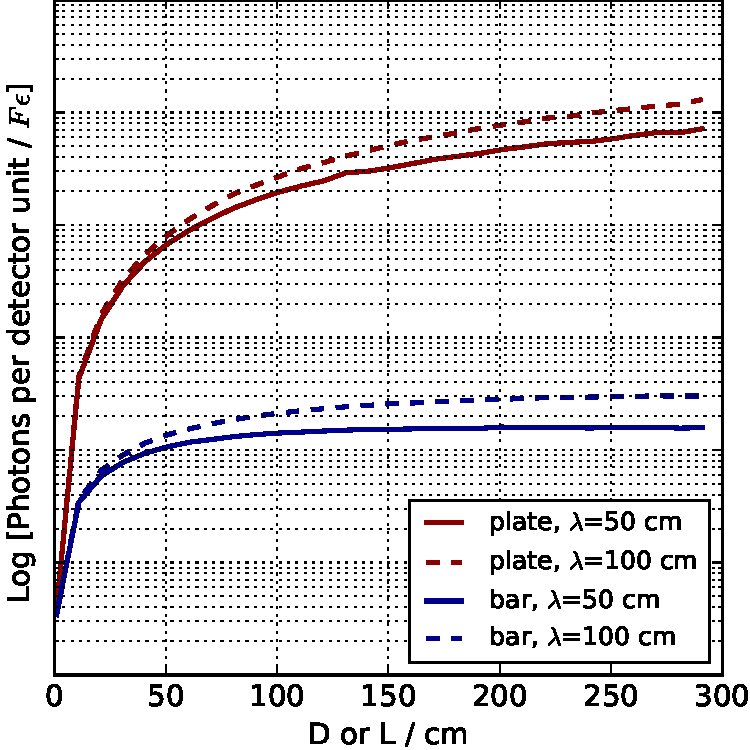
\includegraphics[width=0.48\columnwidth]{./images/FOM2.pdf}
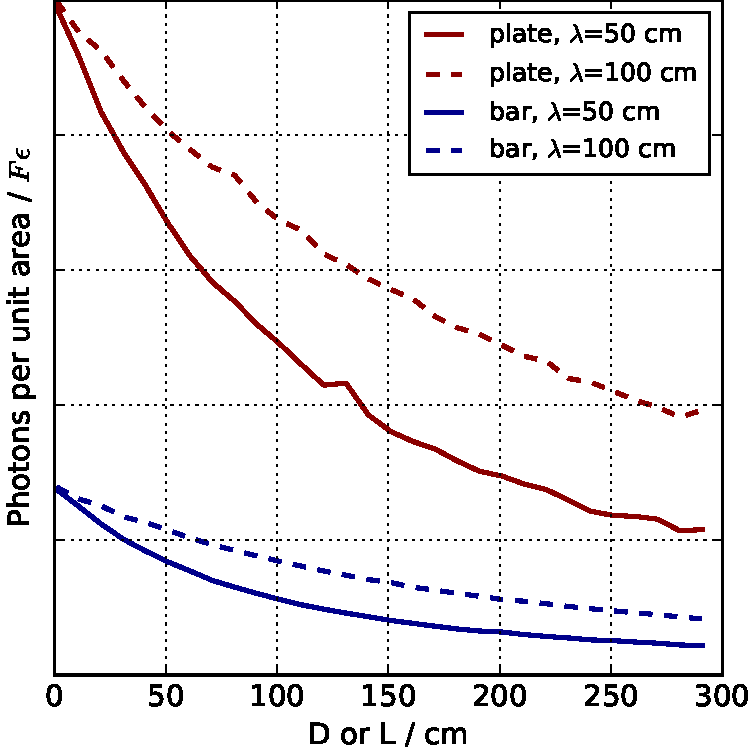
\includegraphics[width=0.48\columnwidth]{./images/FOM3.pdf}
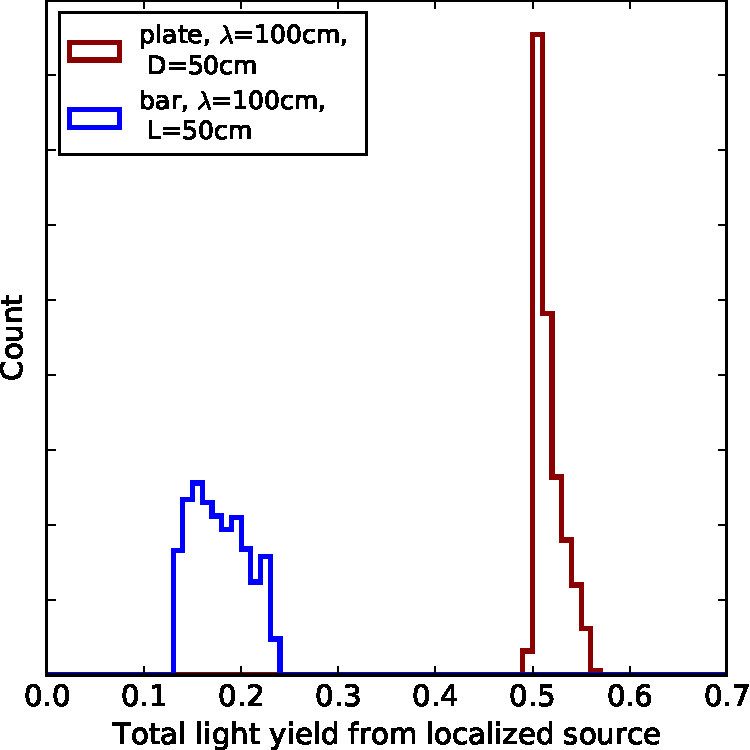
\includegraphics[width=0.48\columnwidth]{./images/FOM4a.pdf}
\par\end{centering}

\caption{Comparison of plate-type to bar-type detectors with various figures of merit described in the text.  The plate significantly outperforms the bar-type detector in all cases. Top left: photons per SiPM. Top right: Photons per detector unit. Bottom left: Photons per unit area. Bottom right: total yield and spread from localized mono-energetic sources. \label{fig:FOMs}}
\end{figure}



\begin{enumerate}
\item For illumination by a distant light source, how many photons can be captured per SiPM?  
\item For illumination by a distant light source, how many photons can be captured per detection unit (one plate or one bar with many coupled SiPMs)?  
\item For illumination by a distant light source, how many photons can be captured per unit surface area?  
\item For localized light deposits at different positions, what is the collection efficiency and how uniform is it?
\end{enumerate}

The parameters of the detector geometry may be optimized differently to satisfy each criterion for both bar and SiPMWheel detectors.  As simplifying assumptions we assume that the thickness of the plastic sheet used to make both the bar and plate is equal to the SiPM width, which we take to be 5mm.  We assume both can be prepared with the same coating quantum efficiency $\epsilon$, are cut from the same material (acrylic with refractive index n=1.5), and that attenuation in the light guide is exponential in light-ray length parallel to the coated surface (this is known to be invalid at very short distances but is a reasonable approximation for longer path lengths \cite{Jones:2013sfa}).  We consider two values of the parallel attenuation length $\lambda$ that appear reasonable based on past studies, $\lambda=50$ cm and $\lambda=100$ cm \cite{Moss:2014ota,Jones:2013sfa}.  Finally we assume that the 5~mm SiPMs are placed with 5~mm spacing between each, which gives three SiPMs per bar, or as many as can fit around the radius of the plate detector.  The FOMs above are compared using the output of a simple ray tracing simulation.

FOM (1) is compared in Figure~\ref{fig:FOMs}, top left.   For both detector types, the collection efficiency increases as the device becomes larger, saturating at a distance comparable to the attenuation length, as expected.   The plate-type detector has consistently higher collection efficiency and a higher saturated value.  This is primarily due to the loss of supercritical rays in the bar detector, which the plate detector does not suffer from.

Whether the most useful Figure~of merit is the light yield per channel or the light yield per detector unit depends on which factor is limiting in the experimental design or budget.  A moderate improvement in FOM (1) corresponds to an enormous improvement in FOM (2) because each plate detector has a large number of SiPM channels, whereas each light guide detector has only 3. This comparison is shown in Figure~\ref{fig:FOMs}, top right (note log scale).  The improvement in FOM (3), the light collected per unit area, is intermediate between these two cases, and is shown in Figure~\ref{fig:FOMs}, lower left.  In all cases, our proposed detector represents a major improvement.

FOM (4), the stability of the light yield for light at different locations, is quantified in Figure~\ref{fig:FOMs}, lower right, which shows example total light yield distributions for localized deposits in random positions across a device with 50 cm length / diameter and 100 cm attenuation length.   Note that no photon counting fluctuations are included in these distributions - they show only the changing light yield due to differences in the detector response in different locations.  Though much improved over the bar-type detector, the energy resolution obtained by simply integrating photons is still not sufficient for sub-\% precision calorimetry.  However, the light yield is correlated with the light source position, which in the case of the SiPMWheel, can be extracted from the distribution of light between SiPMs.  The position resolution and hence the quality of the correction depend strongly on the number of photons detected, and will vary between applications, improving into the sub-percent regime as the detected photon count becomes increasingly large.  The quality of this correction and the optimal method for applying it is something we plan to explore in both simulation- and hardware-based studies if this proposal is funded.




\section{Electroluminescent TPC use case: The NEXT Experiment}

The NEXT collaboration is a primarily US-European collaboration with the goal of developing a ton-scale, ultra-low-background neutrinoless double beta decay detector using high pressure $^{136}$Xe gas (GXe) as the active medium.  This technology has energy resolution far surpassing other xenon-based detectors, and a reconstructable topological signature for neutrinoless double beta decay events which is absent in liquid xenon (LXe) or xenon-doped liquid scintillator (LSXe).  The projected background indices, which will ultimately limit experimental sensitivity at the ton scale, are 9 counts per ton per year per ROI (ctyR) for GXe, 130 ctyR for LXe and 210 ctyR for LSXe, as assessed by an independent review \cite{LRP}.

The NEXT detector is based on an electroluminescent TPC concept. Ionization charge is drifted towards a high-field region where it is amplified through nearly fluctuation-less electroluminescent gain.  Each electron is accelerated in the field of the amplification region, creating excited xenon atoms which decay radiatively, emitting 175 nm light.  This light is collected by two subsystems. Directly behind the electroluminescent region is a tracking array of SiPMs on a 1~cm grid.  These record an image of the amplified event and allow for event topological reconstruction.  Their placement is sufficiently sparse that the integrated light yield per MeV depends on the precise geometry of the event too strongly to provide a calorimetric measurement with the required precision of $\sim$1\% FWHM - this is shown schematically in Figure~\ref{fig:TrackingEffect}, top left.  Addition of more SiPMs to give a complete tiling is possible but costly.  Even if this were implemented, the dark rate of the many SiPMs would like produce fluctuations in the measured energy that prevent intrinsic resolution from being achieved.  

To circumvent this limitation, in the present generation of the NEXT detector, the calorimetric reconstruction of the event is handled by a different subsystem consisting of low-radioactivity PMTs at the cathode end.  Light emitted in the electroluminescent region is reflected around the detector by PTFE foils and shifted to the blue by TPB coatings, and detected by the PMTs of the``energy plane''.  With this arrangement, energy resolutions corresponding to  0.63\% FWHM at Q$_{\beta\beta}$ have been demonstrated \cite{Alvarez:2012yxw}.  A sketch is shown in Figure~ \ref{fig:PlateDetectorNEXT}, top.




\begin{figure}[t]
\begin{centering}
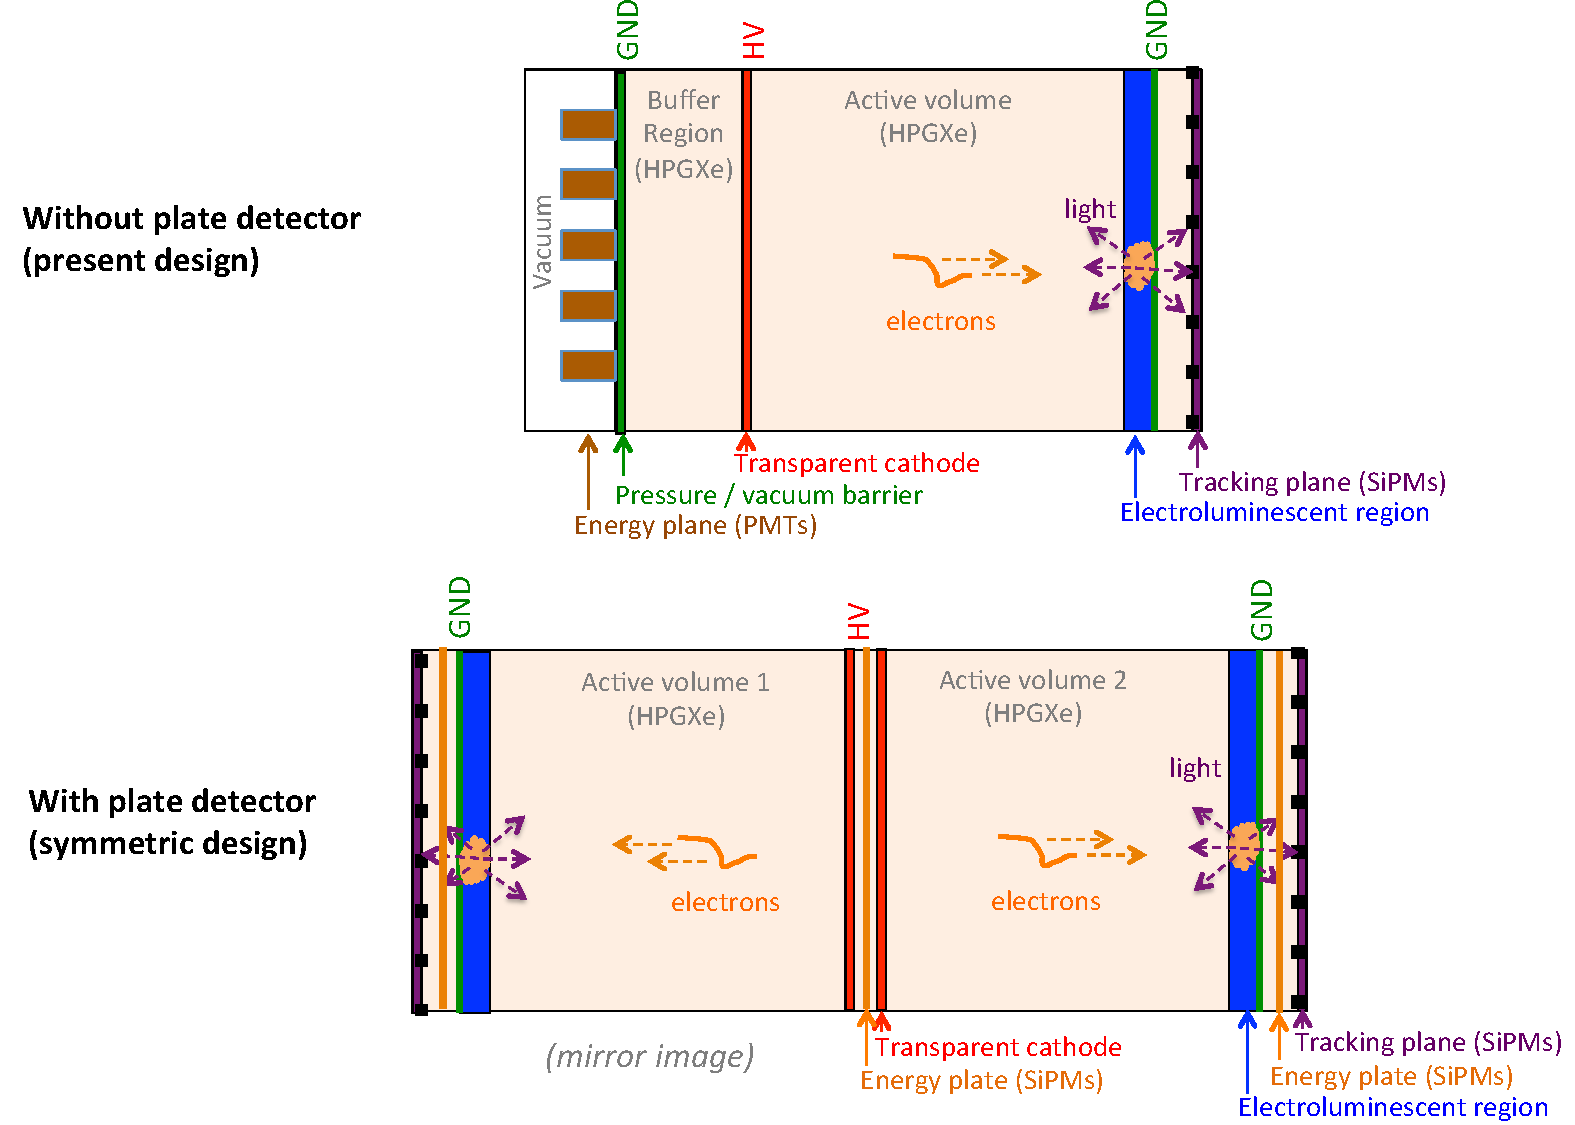
\includegraphics[width=0.85\columnwidth]{./images/PlateDetectorNEXT.pdf}
\par\end{centering}

\caption{Left: Existing asymmetric TPC design, where energy must be recorded using the PMT-based ``energy plane''.  Right: Symmetric design that could be realized using a high-resolution "plate detector".  Plate detectors may be deployed at the anode region, the cathode region, or both. \label{fig:PlateDetectorNEXT}}
\end{figure}


This two-plane solution is not without drawbacks. Even the low radioactive photomultiplier tubes represent a significant fraction of NEXT-100's radioactivity budget, contributing approximately 0.4 counts per ton per keV per year in each of bismuth at thallium backgrounds at Q$_{\beta\beta}$, representing the largest absolutely measured background contribution.  The PMTs must be operated outside of the high-pressure region which introduces an engineering challenge, requiring an evacuated volume to be optically coupled to the active region at 15 bar. Finally, the PMTs must be operated in a low-field region which leads to the HV being graded down in a short ``buffer region'', wasting valuable xenon mass and introducing a region of larger HV stress.

A highly efficient calorimetric plate detector as we have described would allow a significant improvement to the NEXT design.  Instead of measuring energy at the cathode, a wavelength-shifting plate between the electroluminescent mesh and the tracking plane could be used to integrate light emission from the mesh. Since the plate has a uniform collection surface,  dependencies of the light yield on event geometry does not spoil its resolution, as shown in Figure~ \ref{fig:TrackingEffect}, bottom left.  The light which is not guided into the plate escapes through the back surface to be used for tracking.  The plate also provides a focussing effect shown in Figure~\label{fig:TrackingEffect}, right, removing high-angle rays from electroluminescence and potentially improving the tracking resolution of the detector.  It is also plausible to add another energy plane detector behind the cathode transparent cathode. This adds the electrical complications of  SiPMs being operated at high voltage, but increases the calorimetric area by a factor of two.  Finally, because the vacuum region and buffer region are no longer necessary, this design allows a symmetric TPC to be realized, using the GXe volume in a highly efficient way and simplifying the delivery of HV.  This concept is shown in Figure~\ref{fig:PlateDetectorNEXT}, bottom.




\begin{figure}[t!]
\begin{centering}

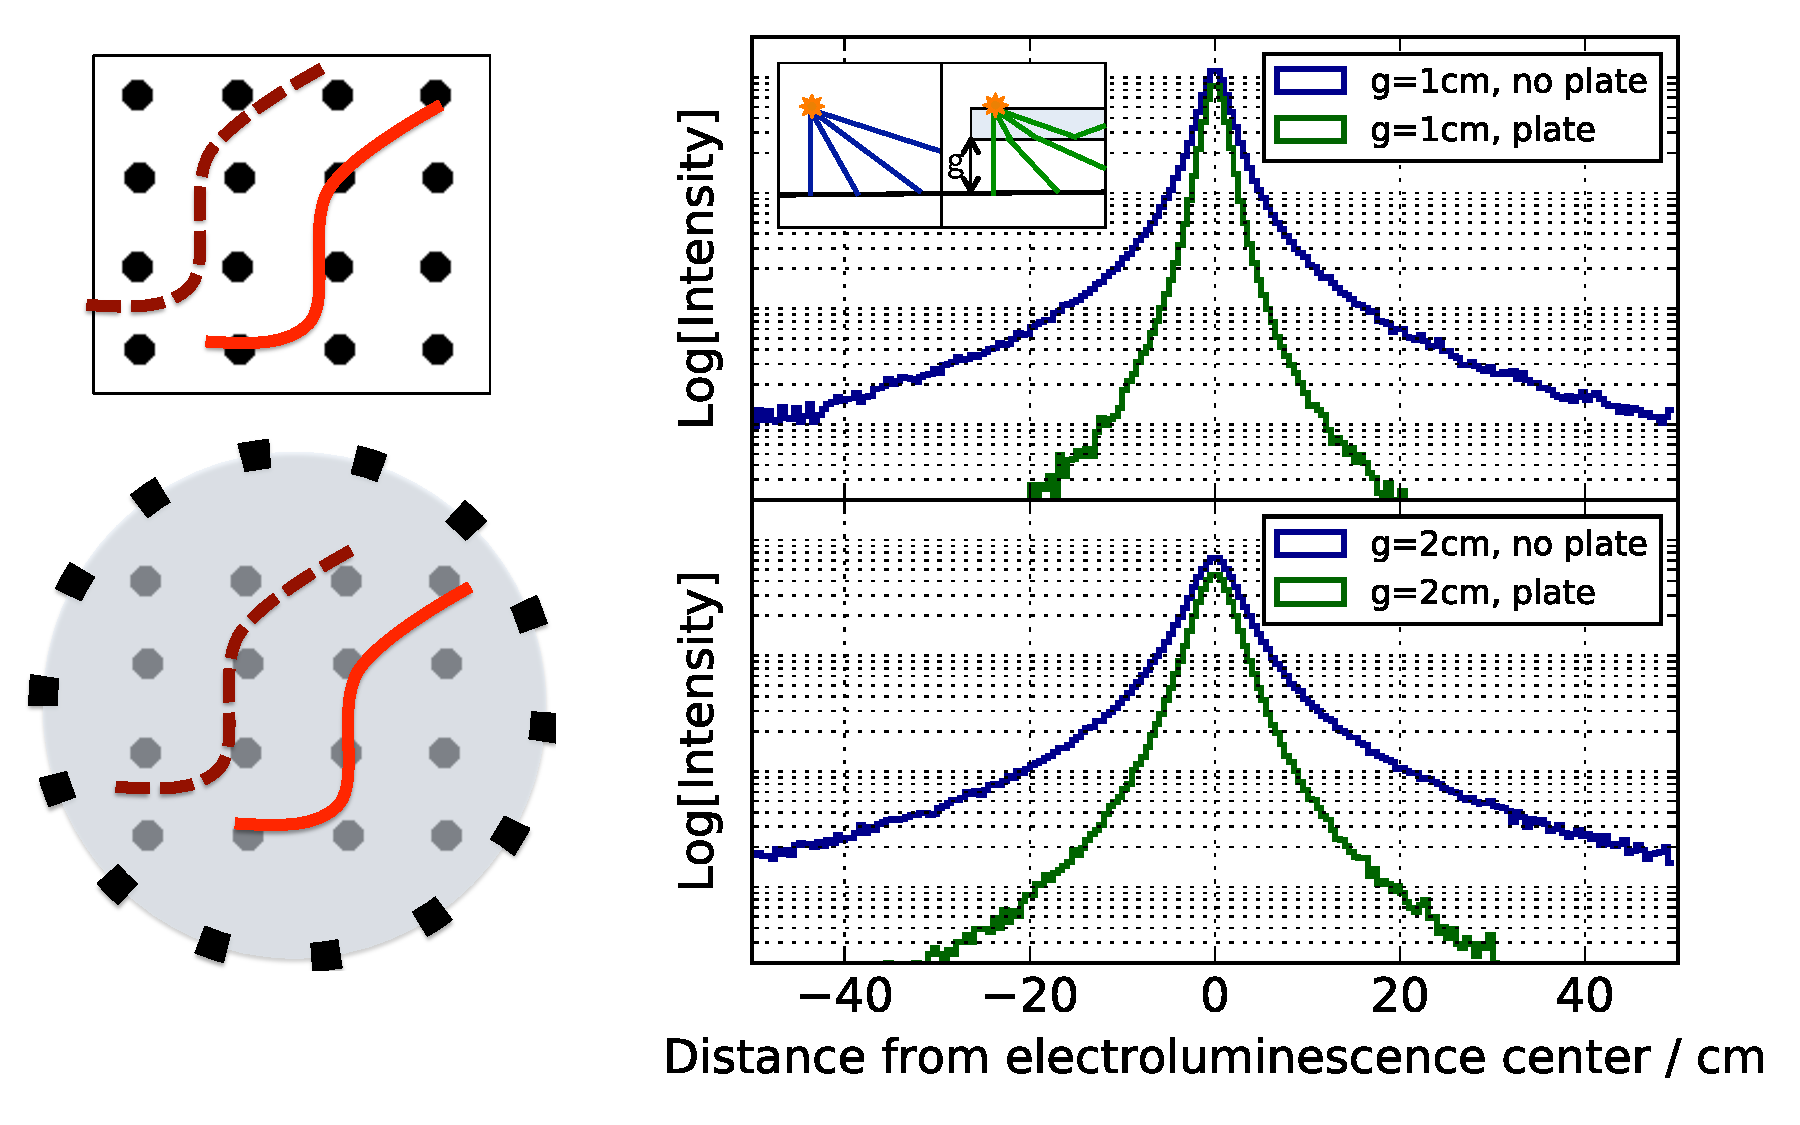
\includegraphics[width=0.85\columnwidth]{./images/FocussingEffectAndTrackShape.pdf}
\par\end{centering}

\caption{Left: Track energy measurement with tracking plane only (top), and tracking plane + plate (bottom).  Right: Focussing effect of plate on transmitted electrolumiscence light, which may improve tracking resolution in NEXT. \label{fig:TrackingEffect}}

\end{figure}

\section{Single-phase LArTPC use case: DUNE}

Light collection in surface-based TPCs plays a critical role of identification of cosmogenic backgrounds which would swamp true neutrino events in the absence of an optical trigger \cite{MicroBooNECosmic}. In deep underground detectors like DUNE, where cosmogenic backgrounds are much reduced, the main goal of light collection systems is fundamentally different. Rather than being primarily a tool to reject energetic off-beam cosmic ray events, the light collection system allows extension of the physics program to low energy, non-beam physics.

The importance of light collection for non-beam physics is primarily related to establishing the position of the event in the drift direction.  This is vital in order to apply a lifetime correction and thus obtain a well calibrated energy for the event from the TPC.  Most of the off-beam neutrino physics goals of DUNE rely on energy reconstruction, either to identify the signal events or to learn about the physics of their sources.

The following are cases where a sensitive light collection system is vital for achieving the physics goals of DUNE:

\begin{itemize}
\item \emph{Detection of supernova neutrinos} \cite{Ankowski:2016lab}.  A high efficiency for detecting 5 MeV electrons has been cited as the detector goal for adequately performing this physics.  This is to be contrasted to the design goal of the MicroBooNE optical system, the largest running LArTPC optical system in the USA, which was to efficiently trigger on 40 MeV protons across the (much smaller) fiducial volume.  Clearly, to meet DUNE's ambitious off-beam physics goals, high light-yield technologies surpassing existing systems are required.
\item \emph{Studies of solar neutrinos with DUNE} \cite{Kudryavtsev:2016ybl} have been discussed. This also requires sensitivity to few-MeV energy deposits across the fiducial volume, with the physics capability extending as the achievable trigger threshold is reduced.  This physics will be greatly enhanced by any improvement in light collection efficiency.
\item \emph{Proton decay} \cite{Adams:2013qkq}.  Golden chanels for proton decay in DUNE include $p \rightarrow K^+ \nu$, $p \rightarrow K^0 \mu^+$ and $p \rightarrow K^+ \mu^- \pi^+$.  Detecting these modes requires not only to trigger on the off-beam events (likely not too challenging due to the large Q-value in the decays), but also identification of the kaon and muon daughters.  Reliable identification is difficult with the TPC alone, since in many cases the ``kink'' in the outgoing track where the daughter particle decays is not strongly pronounced.   It is thus of benefit to access the detailed time-structure of the event, and reconstruct the muon, and potentially even kaon events in time.  A high collection efficiency with the optical system may allow this temporal reconstruction.
\end{itemize}

The present baseline design for the DUNE optical system is a system based on bar detectors.  We have shown in Section \ref{sec:concept} that the SiPMWheel is expected to improve upon the collection efficiency of similarly prepared bars when measured either per-SiPM, per-unit-area, or per-detector.    The SiPMWheel also provides positional information - this will be valuable in cases where multiple events arrive within one drift window, as, for example, during the initial peak of flux from a nearby supernova.  As with bars, the installation of SiPMWheels between mostly-transparent anode plane assemblies is possible as a deployment strategy.   Two-side-coated as well as one-side-coated devices are also possible for this application.

\section{Proposed program of work}

The request in this proposal is primarily for personnel to develop this technology using already existing resources.  We hope to acquire funding for two graduate students who will spend 50\% of their research time for 3 years.  The other 50\% of each will be dedicate to analysis work and funded from other sources.   One undergraduate will also support the team.

In the first year, development will focus on bench-top work, not involving noble element test stands.   This includes learning to produce high quality optical coatings and testing them for efficiency and attenuation length in air, closely following and improving upon previous work with bar coatings (student 1, working primarily with Jones); and commissioning  of a DAQ system capable of reading out large SiPM arrays and efficiently processing the data from these (student 2, working primarily with Asaadi).  Possible improvements beyond the present state-of-the-art include the addition of coating stabilizing additives to improve fluorescence yield and the exploration of high refractive index polymers. Simulation topics relating to detector optimization and expected performance will be instigated as an undergraduate project in the first year.  In the second year, bench-top experience will transition into noble element environments;  with Nygren and Jones, one graduate student will build a subsystem as part of an existing high pressure xenon gas test stand whereby localized electroluminescent emission can be produced near the SiPMWheel surface at various positions to study its energy and position resolution.   The other student will work with Asaadi to integrate the SiPMWheel detector with his planned liquid argon calibration test stand, where an independent program of work to deploy radioactive calibration sources in large liquid argon TPCs will already be underway.  With these sources, the plate performance in liquid argon will be studied.  The undergraduate will assist with one or both activities.  The final year will involve a program of optimization of the detector, potentially along separate trajectories for use in LAr and GXe.  At the end of the three year program we hope to have demonstrated strong energy- and position-reconstruction performance and suitability of the SiPMWheel as both an electroluminescence and primary scintillation light detector.
